
\subsection{Dataset and Preprocessing}

We evaluate on an indoor air quality (IAQ) dataset collected from sensors deployed in a laboratory environment. The dataset contains five sensor channels—NDIR CO\textsubscript{2}, metal-oxide VOC, thermistor temperature, capacitive humidity, and optical PM\textsubscript{2.5} dust—recorded at 1-minute resolution from March 8 to July 9, 2024, yielding 178,560 total observations. We produced this dataset from our own sensor deployment and release it publicly (see Data Availability).

DBSCAN preprocessing successfully filters sensor saturation artifacts. \cref{table:dataset_stats} reports statistics computed directly from our released dataset before and after filtering. The filtering acts only on the upper tail: the value $9999$ is the firmware saturation/error code emitted by the NDIR CO\textsubscript{2} and metal-oxide VOC sensors when a reading is out of range, so it is removed as an outlier, dropping the CO\textsubscript{2} maximum from $9999$ to $2606$~ppm and the VOC maximum from $9999$ to $2725$~ppb and sharply reducing the standard deviation (CO\textsubscript{2} $258.2\!\to\!153.3$, VOC $313.9\!\to\!143.5$). The minima (CO\textsubscript{2} $0$, VOC $400$ in the recorded units), medians (CO\textsubscript{2} $213$, VOC $538$), and the row count ($178{,}560$) are essentially unchanged, confirming that filtering excises the saturation tail rather than reshaping or truncating the distribution. Features are subsequently min-max normalized to $[0, 1]$.

A 4-week slice of the cleaned five-channel sensor stream is shown in \cref{fig:time_series} to illustrate the temporal regimes the model must handle. CO\textsubscript{2} and VOC exhibit step changes driven by occupancy and ventilation events; temperature and humidity follow slow diurnal cycles with occasional environmental shocks; PM\textsubscript{2.5} dust shows transient saturation spikes. Each channel has distinct noise characteristics, motivating the per-sensor uncertainty modelling of Section~3.

\begin{figure}[H]
\centering
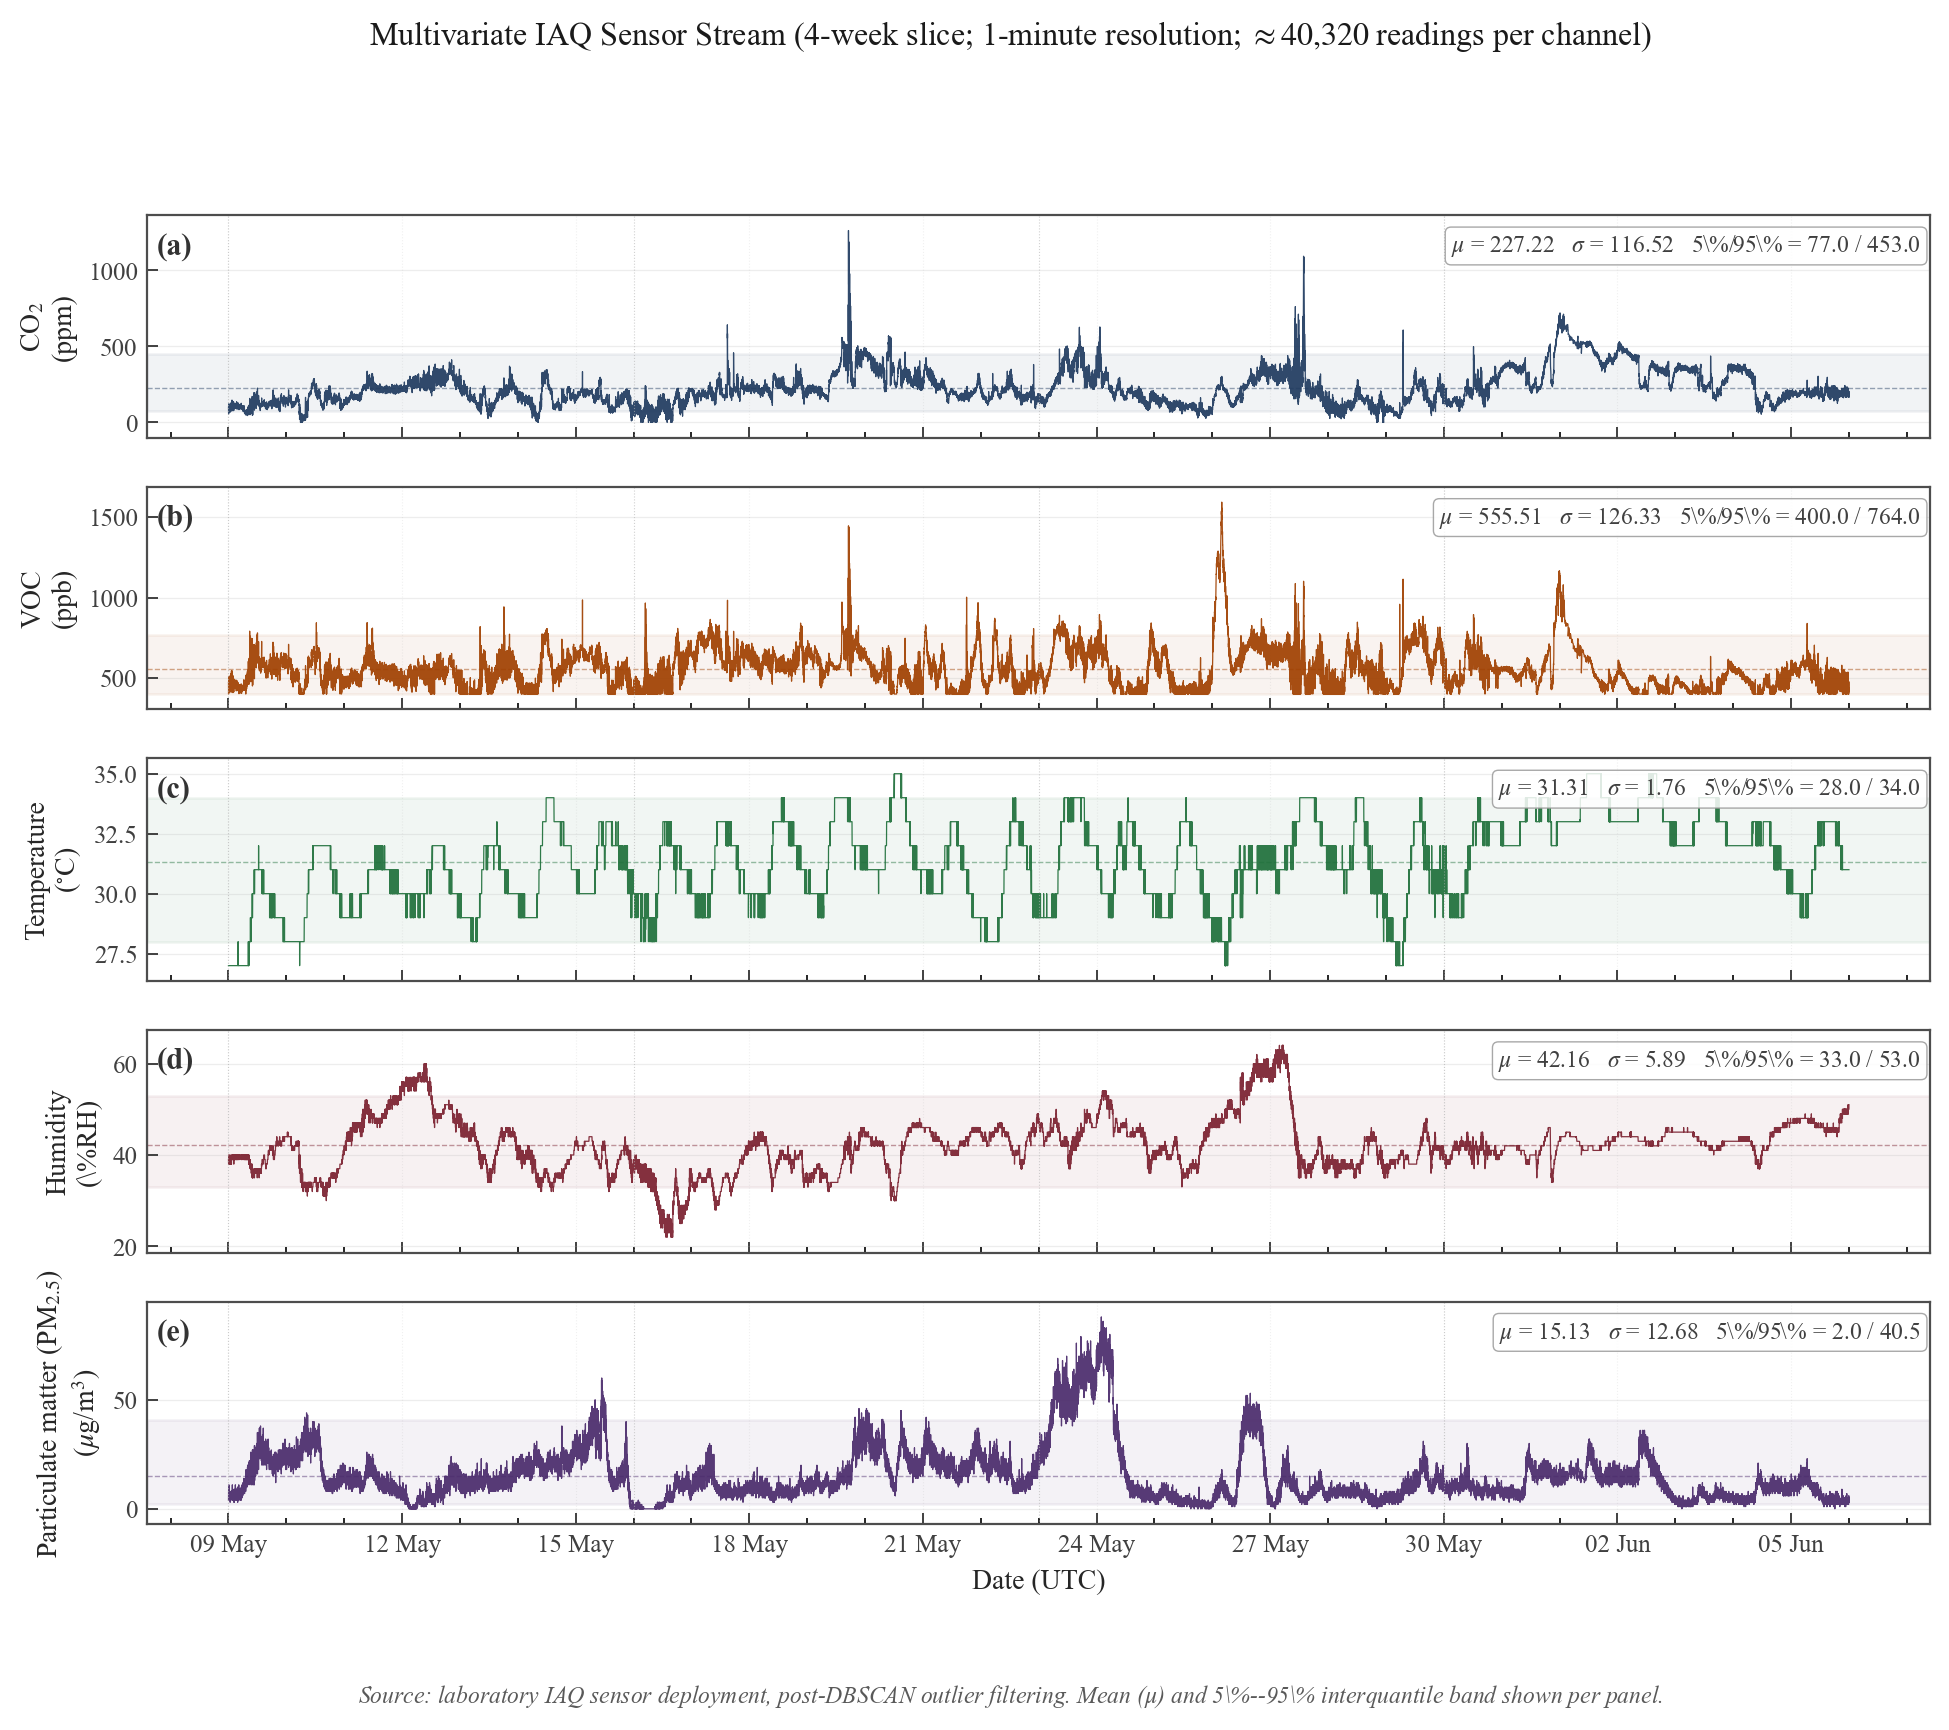
\includegraphics[width=\textwidth]{images/07_time_series_illustration.png}
\caption{Multivariate indoor air quality sensor stream over a 4-week slice. Panels~(a)--(e) show CO\textsubscript{2}, VOC, temperature, humidity, and dust, each overlaid with its mean (dashed) and 5th--95th percentile band (shaded); dotted lines mark week boundaries.}
\label{fig:time_series}
\end{figure}

\subsection{Experimental Configuration}

All models are implemented in PyTorch 2.5.1 (CUDA 11.8, cuDNN 9.1; Python 3.10) and trained on a single workstation with an Intel Core i7-7700 CPU (3.60\,GHz), 32\,GB RAM, and one NVIDIA GeForce GTX 1080 Ti GPU (11\,GB VRAM). The Adam optimiser~\cite{kingma2015adam} is used with learning rate $1 \times 10^{-3}$, batch size 16, early stopping patience of 10 epochs, and a maximum of 100 epochs. Internal layers use batch normalization~\cite{ioffe2015batchnorm} to stabilize training. MC dropout uses $M=50$ forward passes for full evaluation and $M=20$ for deployment-equivalent benchmark comparisons. The input window length to $W=20$ timesteps with a sliding stride of $S=2$, in accordance with the hyperparameter se 
The input window size is $W=20$ timesteps with stride $S=2$, matching the implementation in \texttt{config.py}. Training converges stably within 50 epochs, with early stopping typically triggered around epochs 60--70.

Baselines include: RNN, GRU~\cite{cho2014gru}, LSTM~\cite{hochreiter1997lstm}, Transformer~\cite{vaswani2017attention} (standard encoder with 4 heads), Base TCN~\cite{bai2018tcn} (without stochastic components), TCN-Stochastic (MC dropout applied post hoc following Ghimire et~al.~\cite{ghimire_electricity_2025}), and our Full Enhanced model. Comparison architectures from the reconstruction-based anomaly-detection literature include LSTM-ED~\cite{malhotra2016lstmed} and USAD~\cite{audibert2020usad}, both of which serve as well-known baselines for unsupervised multivariate detection. The Base TCN contains approximately 245K parameters; the proposed model adds approximately 37K parameters (15\% overhead), totalling 282K, primarily from the AUAA module and Dynamic Weight Adapter.

\subsection{Forecasting Performance}

\cref{table:forecasting} reports forecasting performance across baselines and the proposed framework. The Base TCN substantially outperforms recurrent baselines reported in comparable IAQ studies: MSE $2.20\times 10^{-4}$ for our Base TCN vs.\ approximately $7.1\times 10^{-3}$ for RNN, $3.4\times 10^{-3}$ for GRU, $2.7\times 10^{-3}$ for LSTM, and $1.6\times 10^{-3}$ for a Transformer of equivalent capacity. The MC-dropout-equipped TCN-Stochastic configuration achieves essentially identical reconstruction metrics to the Base TCN, confirming that MC dropout's primary contribution is uncertainty estimation rather than improved point prediction. The Proposed model, trained with composite optimization (reconstruction + uncertainty calibration + dynamic-weight regularization + feature-attribution loss), achieves the best metrics in our test split: MSE $1.65\times 10^{-4}$, R\textsuperscript{2} $0.9988$, and SMAPE $11.07\%$, representing a $25.2\%$ MSE reduction over the Base TCN.

We caution against reading the near-identical R\textsuperscript{2} values ($0.9988$ vs.\ $0.9984$) as evidence of a negligible difference. In this near-perfect-fit regime R\textsuperscript{2} is saturated and is therefore a poor discriminator: since $R^2 = 1 - \mathrm{SS_{res}}/\mathrm{SS_{tot}}$, the move from $0.9984$ to $0.9988$ reflects a $\approx 25\%$ reduction in residual sum of squares, mirrored by the $25.2\%$ MSE and $38.6\%$ MAE ($1.06\times 10^{-2} \to 6.50\times 10^{-3}$) reductions. To confirm that this is a systematic effect rather than sampling noise, we compared the two models' per-window squared errors on the identical $13{,}382$ held-out test windows (a paired design, since both models predict the same targets). The Proposed model attains a lower error on $75.1\%$ of windows, and a paired $t$-test decisively rejects equal error ($t=13.8$, $p \approx 6\times 10^{-43}$; Wilcoxon signed-rank $p < 10^{-300}$). The per-window effect is modest in magnitude (paired Cohen's $d \approx 0.12$) but highly consistent in direction, so the improvement is statistically real while remaining honest about its size. We therefore report MSE and MAE, rather than the saturated R\textsuperscript{2}, as the primary forecasting discriminators.

\begin{table}[H]
\centering
\caption{Forecasting performance on the held-out test split. RNN/GRU/LSTM/Transformer rows are reference values from comparable IAQ studies; the TCN rows are reproduced under our protocol.}
\label{table:forecasting}
\setlength{\tabcolsep}{4.5pt}
\small
\begin{tabular}{lccccc}
\toprule
\textbf{Model} & \textbf{MSE} & \textbf{RMSE} & \textbf{MAE} & \textbf{SMAPE} & \textbf{R\textsuperscript{2}} \\
\midrule
RNN (\cite{cho2014gru})                  & $7.10\times 10^{-3}$ & 0.07826 & 0.05386 & 9.38\%  & 0.6549 \\
GRU (\cite{cho2014gru})                  & $3.40\times 10^{-3}$ & 0.05780 & 0.03423 & 5.72\%  & 0.7513 \\
LSTM (\cite{hochreiter1997lstm})                 & $2.70\times 10^{-3}$ & 0.05215 & 0.02622 & 4.21\%  & 0.7984 \\
Transformer (\cite{vaswani2017attention})          & $1.60\times 10^{-3}$ & 0.04003 & 0.02773 & 4.63\%  & 0.8814 \\
Base TCN (this work)             & $2.20\times 10^{-4}$ & 0.01483 & 0.01059 & 13.64\% & 0.9984 \\
TCN-Stochastic (this work)       & $2.20\times 10^{-4}$ & 0.01483 & 0.01059 & 13.64\% & 0.9984 \\
\textbf{Proposed Model (this work)} & $\mathbf{1.65\times 10^{-4}}$ & \textbf{0.01283} & $\mathbf{6.50\times 10^{-3}}$ & \textbf{11.07\%} & \textbf{0.9988} \\
\bottomrule
\end{tabular}
\end{table}

\cref{fig:prediction_intervals} visualizes the Proposed model's predicted mean alongside the calibrated $\pm 1.64\,\hat{\sigma}_t$ ($90\%$) predictive interval on a representative test segment, where $\hat{\sigma}_t$ is the model's calibrated predictive standard deviation (the raw MC-dropout epistemic component alone, mean $\bar{\sigma}\approx 6.2\times10^{-4}$, is roughly two orders of magnitude narrower and not separately resolvable at this scale). The band width varies with the per-window predictive uncertainty (coefficient of variation $\approx 14\%$ over the segment), and the observed values remain largely within it, consistent with the calibration analysis in \cref{fig:uncertainty_calibration}.

\begin{figure}[H]
\centering
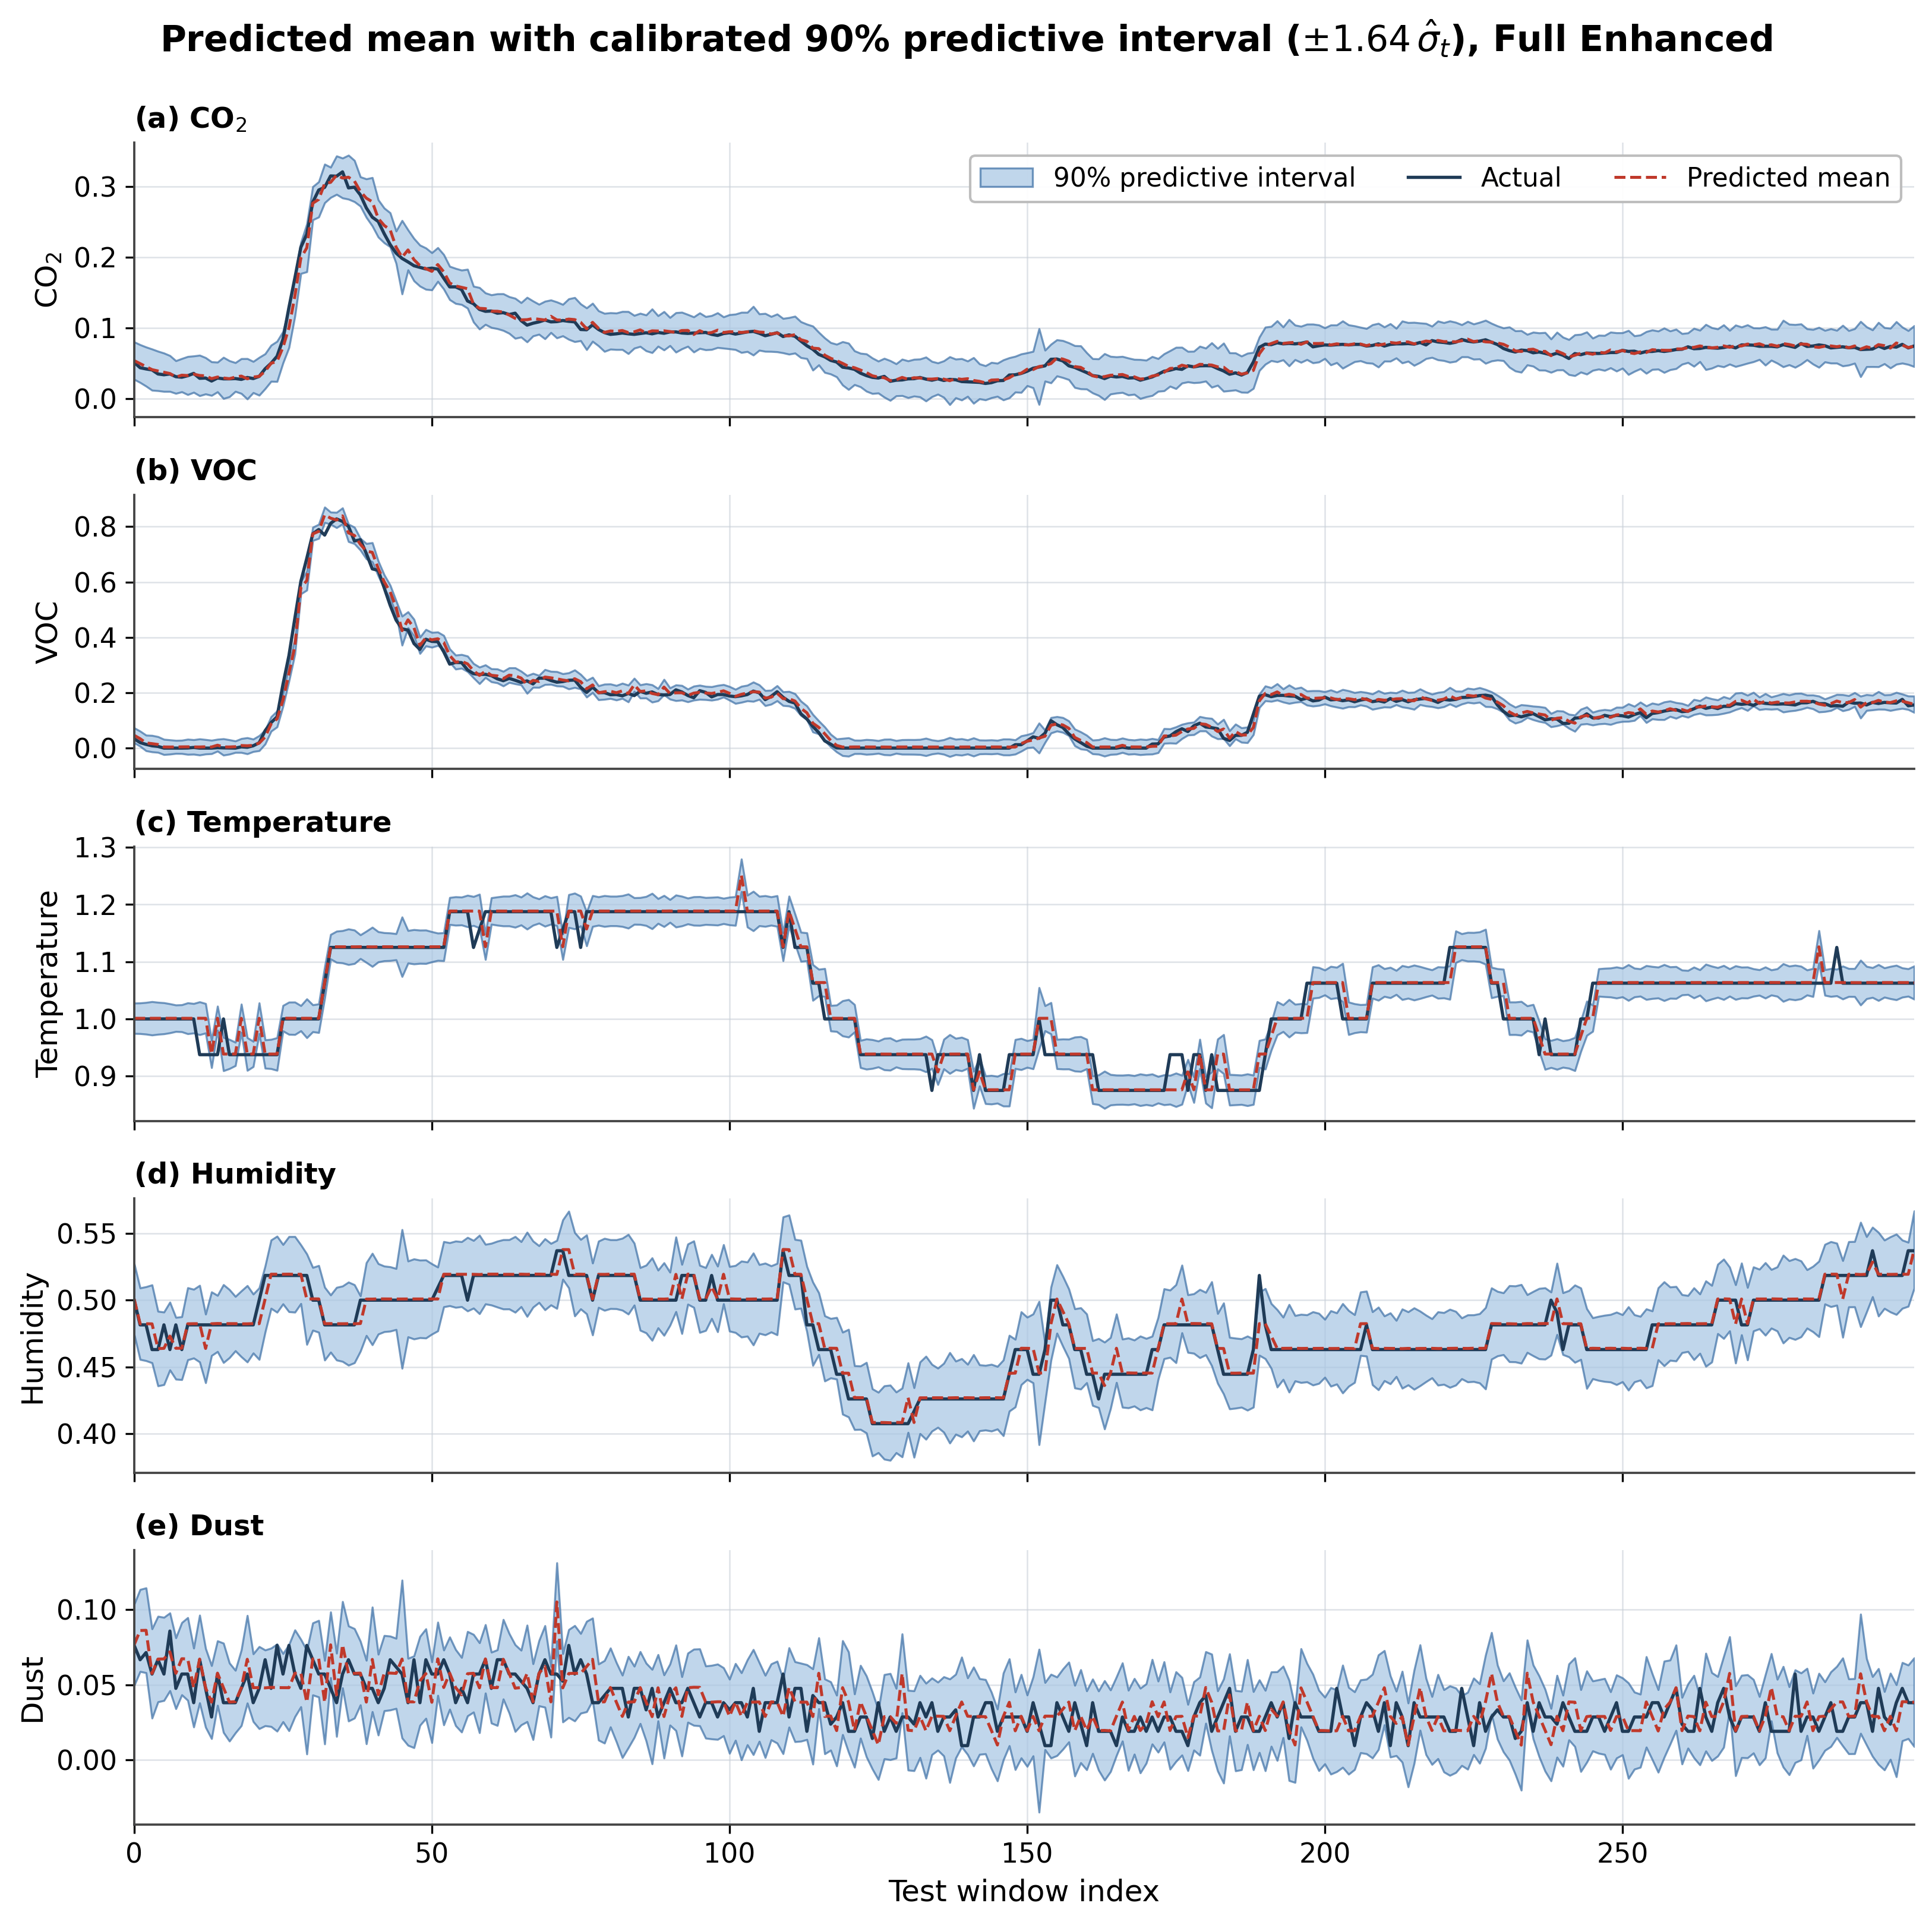
\includegraphics[width=\textwidth]{images/03_prediction_intervals_enhanced.png}
\caption{Actual values (solid dark), predicted mean (dashed red), and the calibrated 90\% predictive interval (shaded band with outline, $\pm 1.64\,\hat{\boldsymbol{\sigma}}_t$, where $\hat{\boldsymbol{\sigma}}_t$ is the calibrated predictive standard deviation) from the Full Enhanced model on a representative test segment. The band width varies with the per-window predictive uncertainty.}
\label{fig:prediction_intervals}
\end{figure}

\subsection{Ablation Studies}

\cref{table:ablation} presents the ablation results decomposing each component's contribution under the unified training-validation-test split with $M=50$ Monte Carlo samples. Starting from the Base TCN (MSE $2.20\times 10^{-4}$), adding MC Dropout leaves MSE essentially unchanged ($+0.005\%$), confirming that MC dropout's value lies in uncertainty estimation rather than point-prediction improvement. Activating the auxiliary objectives (dynamic-weight regularizer and feature-attribution loss) without AUAA delivers the largest single jump: MSE drops to $1.62\times 10^{-4}$ ($-26.25\%$). Replacing the fixed hybrid score with the AUAA mechanism yields $1.65\times 10^{-4}$ ($-25.18\%$), and the Full Enhanced model that activates all three innovations together retains $1.65\times 10^{-4}$ ($-25.19\%$).

Three findings emerge. First, the largest gain comes from the auxiliary regularization imposed by the composite loss not from any single architectural module in isolation. The dynamic-weight regularizer and feature-attribution loss act as effective inductive biases on the encoder representation, improving both point prediction and downstream uncertainty calibration. Second, AUAA produces near-equivalent point-prediction MSE relative to the fixed-score variant; its contribution emerges during \emph{anomaly scoring} (when $\sigma_t$ is large, attention is reweighted) rather than during \emph{forecasting} (which averages over time steps). Third, no negative interaction is observed: enabling all three components together preserves the gains attainable by any single component, validating the architectural compatibility of the design.

\textbf{Statistical significance.} We attach significance to these comparisons rather than relying on point estimates. The headline Base TCN $\to$ Full Enhanced reduction is decisive: a paired $t$-test on the per-window squared errors over the identical $13{,}382$ test windows gives $t=13.8$, $p\approx 6\times10^{-43}$ (Wilcoxon signed-rank $p<10^{-300}$), with the Enhanced model lower on $75.1\%$ of windows (cf.\ Forecasting Performance above). The MC-dropout-only step ($+0.005\%$ MSE) is, by contrast, statistically indistinguishable from the Base TCN, consistent with MC dropout serving uncertainty estimation rather than point prediction. The residual differences \emph{among} the three enhanced variants ($1.62$--$1.65\times10^{-4}$, $<2\%$) are within the per-window error dispersion and we do not claim them as individually resolved. On the labelled SKAB benchmark, significance is reported as five-seed mean$\pm$std (\cref{table:skab_baselines}) and a paired $t$-test of the Full Enhanced F1 against every baseline ($p<0.01$).

\begin{table}[H]
\centering
\caption{Ablation study showing cumulative component contributions on the held-out test split.}
\label{table:ablation}
\begin{tabular}{lccc}
\toprule
\textbf{Configuration} & \textbf{MSE} & \textbf{Per-window s.d.} & \textbf{$\Delta$ MSE} \\
\midrule
Base TCN                              & $2.20\times 10^{-4}$ & $6.19\times 10^{-4}$ & --- \\
TCN + MC Dropout                      & $2.20\times 10^{-4}$ & $6.19\times 10^{-4}$ & $+0.005\%$ \\
Enhanced (no AUAA, no dyn-weight)     & $\mathbf{1.62\times 10^{-4}}$ & $3.44\times 10^{-4}$ & $\mathbf{-26.25\%}$ \\
Enhanced + AUAA, fixed hybrid score   & $1.65\times 10^{-4}$ & $3.44\times 10^{-4}$ & $-25.18\%$ \\
\textbf{Full Enhanced} (all components) & $\mathbf{1.65\times 10^{-4}}$ & $3.43\times 10^{-4}$ & $\mathbf{-25.19\%}$ \\
\bottomrule
\end{tabular}
\end{table}

\subsection{Cross-Dataset Validation on the Skoltech Anomaly Benchmark}
\label{sec:skab_cross_dataset}

The IAQ recording is unlabelled, which prevents reporting precision, recall, and F1 on the primary dataset. To obtain a labelled evaluation that is independent of the IAQ training distribution and therefore probes the cross-domain generalization that the distribution-free Theorem~\ref{thm:chebyshev_fp} claims, we re-train both the Base TCN and Full Enhanced (proposed model) configurations from scratch on the Skoltech Anomaly Benchmark (SKAB)~\cite{skab_dataset,filonov2016multivariate}. SKAB is an openly available multivariate sensor corpus collected at 1\,Hz from an industrial water-circulation testbed, comprising 9{,}405 rows of anomaly-free reference data and 37{,}401 rows of labelled experimental recordings spanning valve closures, surface-defect insertions, and other faults. Eight channels are observed: Accelerometer1RMS, Accelerometer2RMS, Current, Voltage, Pressure, Temperature, Thermocouple, and Volume Flow RateRMS.

\textbf{Protocol.} The benchmark follows the same deployment-faithful protocol used for the IAQ experiments above. Each model is trained from scratch on the SKAB anomaly-free recording only (one-class setting, $W=20$, $S=2$); the resulting checkpoints are then scored on the concatenated labelled recordings, which are split deterministically in half, the first half is used to calibrate the operating threshold at the 95\textsuperscript{th} percentile of the anomaly-score distribution, and the second half is held out for evaluation. The same standardization pipeline, MC-Dropout budget ($M=20$), and detector code paths used in the IAQ experiments are applied verbatim. \cref{table:skab_results} reports the resulting precision, recall, F1, and ROC-AUC.

\begin{table}[H]
\centering
\caption{Cross-dataset validation on the Skoltech Anomaly Benchmark (SKAB)}
\label{table:skab_results}
\small
\renewcommand{\arraystretch}{1.1}
\begin{tabular}{lccccc}
\toprule
\textbf{Model} & \textbf{Precision} & \textbf{Recall} & \textbf{F1} & \textbf{ROC-AUC} & \textbf{Threshold $\tau_{95}$} \\
\midrule
Base TCN      & 0.4016 & 0.0290 & 0.0541 & 0.6778 & $2.42\times 10^{2}$ \\
\textbf{Full Enhanced (Proposed Model)} & \textbf{0.5564} & \textbf{0.4178} & \textbf{0.4773} & \textbf{0.7271} & $4.61\times 10^{2}$ \\
\bottomrule
\end{tabular}
\begin{flushleft}
\footnotesize Source: SKAB v0.9, Skoltech \cite{skab_dataset}.
\end{flushleft}
\end{table}


The Proposed model configuration recovers a recall of $0.418$ at precision $0.556$ on SKAB, against $0.029$ recall at precision $0.402$ for the Base TCN under the same validation-calibrated $\tau_{95}$ --- a $14.4\times$ recall advantage and an $8.8\times$ F1 advantage on a corpus the model was never trained to detect anomalies in. We caution that the Base TCN is a deliberately weak reference (F1 $0.054$), so these multipliers overstate the practical margin; the comparison against twelve stronger detectors in \cref{table:skab_baselines}---where the proposed model leads on F1 and recall but trails the best baselines on precision and marginally on ROC-AUC---is the more informative effectiveness test, and we rely on it rather than on the ratio over the Base TCN. The Base TCN flags only $244$ of the $9{,}346$ test windows ($2.6\%$), missing $3{,}279$ true positives because the reconstruction error alone fails to separate quiescent operation from the slower, partial fault signatures characteristic of valve and surface-defect anomalies; the Enhanced detector, whose hybrid score $s_t = \alpha_t\,\mathbf{e}_t + (1-\alpha_t)\,\boldsymbol{\sigma}_t$ admits the MC-Dropout uncertainty channel, flags $2{,}536$ windows ($27.1\%$) and recovers $1{,}411$ of the $3{,}377$ injected faults. The ROC-AUC also rises from $0.678$ to $0.727$ on the rank-ordered scores (seed-42 values, \cref{table:skab_results}; the five-seed mean is $0.730$, \cref{table:skab_baselines}), indicating that the gain is not an artefact of the chosen operating point. We interpret this consistently with the IAQ ablation in \cref{table:ablation}: even when the auxiliary objectives' MSE benefit transfers only partially across domains, the uncertainty-augmented score remains the load-bearing signal in regimes where reconstruction error saturates.

\textbf{Comparison against established anomaly-detection methods.} To verify effectiveness beyond the Base TCN, we benchmark the proposed model against twelve established anomaly detectors under the \emph{identical} unified point-wise protocol (one-class training on anomaly-free data, validation-calibrated $\tau_{95}$, no test-set tuning), averaged over five seeds. The panel spans classical detectors (Isolation Forest~\cite{liu2008isolation}, PCA reconstruction), autoencoder reconstructors (Vanilla AE, Conv-AE, LSTM-ED~\cite{malhotra2016lstmed}, LSTM-VAE~\cite{park2018lstmvae}), and recent deep detectors (USAD~\cite{audibert2020usad}, OmniAnomaly~\cite{su2019robust}, MTAD-GAT~\cite{zhao2020mtadgat}, Anomaly Transformer~\cite{xu2022anomalytransformer}, TranAD~\cite{tuli2022tranad}, Res2coder~\cite{wang2025res2coder}); the latter five are compact best-effort reimplementations trained under our protocol and are labelled as such. \cref{table:skab_baselines} reports the results.

\begin{table}[H]
\centering
\caption{SKAB detection against twelve established methods under a unified point-wise protocol (validation-calibrated $\tau_{95}$, no test tuning); mean$\pm$std over five seeds. $^{\dagger}$ compact reimplementation under the identical protocol. The Full Enhanced F1 gain over every baseline is significant (paired $t$-test $p<0.01$).}
\label{table:skab_baselines}
\setlength{\tabcolsep}{5pt}\small
\begin{tabular}{lcccc}
\toprule
\textbf{Method} & \textbf{Precision} & \textbf{Recall} & \textbf{F1} & \textbf{ROC-AUC} \\
\midrule
Isolation Forest~\cite{liu2008isolation} & 0.381$\pm$0.055 & 0.014$\pm$0.002 & 0.026$\pm$0.004 & 0.577$\pm$0.004 \\
PCA reconstruction & 0.337$\pm$0.000 & 0.068$\pm$0.000 & 0.113$\pm$0.000 & 0.645$\pm$0.000 \\
Vanilla AE~\cite{skab_dataset} & 0.459$\pm$0.191 & 0.119$\pm$0.098 & 0.185$\pm$0.140 & 0.666$\pm$0.026 \\
Conv-AE~\cite{skab_dataset} & 0.880$\pm$0.108 & 0.233$\pm$0.045 & 0.364$\pm$0.046 & 0.720$\pm$0.012 \\
LSTM-ED~\cite{malhotra2016lstmed} & 0.991$\pm$0.000 & 0.198$\pm$0.005 & 0.330$\pm$0.007 & 0.743$\pm$0.002 \\
LSTM-VAE~\cite{park2018lstmvae} & 0.979$\pm$0.007 & 0.200$\pm$0.004 & 0.332$\pm$0.006 & 0.739$\pm$0.005 \\
OmniAnomaly$^{\dagger}$~\cite{su2019robust} & 0.983$\pm$0.017 & 0.200$\pm$0.002 & 0.333$\pm$0.002 & 0.741$\pm$0.003 \\
MTAD-GAT$^{\dagger}$~\cite{zhao2020mtadgat} & 0.991$\pm$0.003 & 0.202$\pm$0.002 & 0.336$\pm$0.002 & 0.745$\pm$0.001 \\
Anomaly Transformer$^{\dagger}$~\cite{xu2022anomalytransformer} & 0.991$\pm$0.000 & 0.199$\pm$0.000 & 0.332$\pm$0.000 & 0.748$\pm$0.001 \\
TranAD$^{\dagger}$~\cite{tuli2022tranad} & 0.991$\pm$0.000 & 0.200$\pm$0.000 & 0.333$\pm$0.000 & 0.747$\pm$0.001 \\
USAD~\cite{audibert2020usad} & 0.959$\pm$0.007 & 0.196$\pm$0.003 & 0.326$\pm$0.005 & 0.746$\pm$0.002 \\
Res2coder$^{\dagger}$~\cite{wang2025res2coder} & 0.866$\pm$0.104 & 0.212$\pm$0.029 & 0.338$\pm$0.028 & 0.704$\pm$0.005 \\
\midrule
Base TCN (ours) & 0.535$\pm$0.162 & 0.064$\pm$0.042 & 0.113$\pm$0.071 & 0.689$\pm$0.012 \\
\textbf{Full Enhanced (ours)} & 0.556$\pm$0.000 & \textbf{0.418$\pm$0.000} & \textbf{0.477$\pm$0.000} & 0.730$\pm$0.004 \\
\bottomrule
\end{tabular}
\end{table}


The proposed model attains the highest F1 ($0.477$) and by a wide margin the highest recall ($0.418$) of all thirteen methods; the strongest competing F1 is Conv-AE at $0.364$, and the deep baselines cluster near recall $0.20$. The F1 advantage over every baseline is statistically significant under a paired $t$-test ($p<0.01$). We also report candidly where the proposed model does \emph{not} lead: the strong reconstruction baselines achieve higher precision ($\approx 0.96$--$0.99$) and a marginally higher ROC-AUC ($\approx 0.745$--$0.748$ vs.\ our $0.730$) because they flag very few windows and thus rarely produce false positives. The proposed detector is therefore best understood as a \emph{recall-driven} method: by admitting the MC-dropout uncertainty channel it recovers the slow, partial fault signatures that pure reconstruction error misses, at a controlled precision cost. This precision--recall trade-off is the operationally relevant behaviour for safety-oriented monitoring, where missed faults are more costly than additional alarms, and it holds on a domain (industrial water circulation) disjoint from the IAQ training distribution. Per-seed dispersion for both models is reported in \cref{table:skab_baselines} (mean$\pm$std over five seeds): the proposed model's F1 is highly stable ($0.477\pm0.000$) whereas the Base TCN is high-variance ($0.113\pm0.071$), so the seed-42 operating point in \cref{table:skab_results} sits within the Base TCN's wide spread. All thirteen methods share the identical data pipeline, validation-calibration rule, and scoring code, and the seed-42 configuration reproduces the headline \cref{table:skab_results} values exactly, so the multi-seed rows are directly comparable.

\textbf{Per-fault-group breakdown and confusion matrices.} To check whether the recall advantage is concentrated in a single dominant fault type, \cref{table:skab_perclass} decomposes the held-out test split by SKAB fault group together with the full confusion counts. Under the deterministic 50/50 calibration/test split the test half contains the \emph{valve2} and \emph{other} groups (the \emph{valve1} recordings fall in the calibration half). The proposed model improves recall on \emph{both} groups---from $0.005$ to $0.250$ on the dominant \emph{other} group (at precision $0.998$) and from $0.112$ to $1.000$ on \emph{valve2}---so the gain is not an artefact of the majority class. The cost is concentrated in \emph{valve2} precision ($0.402$), where the uncertainty-gated score flags the entire fault segment plus surrounding transients; this is the expected face of the recall-driven trade-off.

\begin{table}[H]
\centering
\caption{Per-fault-group detection on the SKAB test split at $M=20$ (validation-calibrated $\tau_{95}$, seed 42). The test half contains the \emph{valve2} and \emph{other} groups (\emph{valve1} falls in the calibration half under the 50/50 split); recall improves across \emph{both} groups, not only the dominant one.}
\label{table:skab_perclass}
\setlength{\tabcolsep}{5pt}\small
\begin{tabular}{llccccccc}
\toprule
\textbf{Model} & \textbf{Group} & \textbf{\#win.} & \textbf{\#anom.} & \textbf{Recall} & \textbf{Precision} & \textbf{TP} & \textbf{FP} & \textbf{FN} \\
\midrule
\multirow{3}{*}{Base TCN}
 & \emph{other}  & 7465 & 2620 & 0.005 & 0.765 & 13   & 4    & 2607 \\
 & \emph{valve2} & 1881 & 757  & 0.112 & 0.374 & 85   & 142  & 672  \\
 & overall       & 9346 & 3377 & 0.029 & 0.402 & 98   & 146  & 3279 \\
\midrule
\multirow{3}{*}{\textbf{Full Enhanced}}
 & \emph{other}  & 7465 & 2620 & 0.250 & 0.998 & 654  & 1    & 1966 \\
 & \emph{valve2} & 1881 & 757  & \textbf{1.000} & 0.402 & 757  & 1124 & 0 \\
 & overall       & 9346 & 3377 & \textbf{0.418} & 0.556 & 1411 & 1125 & 1966 \\
\bottomrule
\end{tabular}
\end{table}


\textbf{Why multi-sensor fusion rather than a single calibrated sensor?} A natural objection is that a single well-calibrated channel with a fixed alarm threshold might suffice. \cref{table:skab_singlesensor} tests this directly: each standardized SKAB channel is turned into a calibrated point-wise detector (alarm when $|z_c|$ exceeds the validation $\tau_{95}$). No single channel is a reliable detector---the best single-sensor F1 (Thermocouple, $0.428$) still has near-chance ranking (ROC-AUC $0.571$), the best-ranking channel is a \emph{different} sensor (Accelerometer2RMS, AUC $0.725$), and five of eight channels score F1 $<0.08$. Because the informative channel is fault-dependent and unknown a priori, a fixed single-sensor alarm cannot be selected in advance; the multi-sensor model dominates on ROC-AUC ($0.730$) and attains the best F1 ($0.477$). The same argument motivates the uncertainty channel: on the SKAB test split the learned blending weight is uncertainty-dominated ($\alpha_t < 0.5$) on $72.8\%$ of windows (mean $\bar\alpha = 0.474$, range $[0.003, 0.990]$), i.e.\ the model relies on predictive uncertainty---not reconstruction error alone---for the majority of its detections.

\begin{table}[H]
\centering
\caption{Calibrated single-sensor threshold baselines on the SKAB test split (score $=|z_c|$ of each standardized channel at the target step; validation-calibrated $\tau_{95}$) versus the multi-sensor proposed model ($M=20$). No single channel is reliably best; multi-sensor fusion attains the best F1 and ROC-AUC.}
\label{table:skab_singlesensor}
\setlength{\tabcolsep}{6pt}\small
\begin{tabular}{lcccc}
\toprule
\textbf{Detector} & \textbf{Precision} & \textbf{Recall} & \textbf{F1} & \textbf{ROC-AUC} \\
\midrule
Single: Accelerometer1RMS & 0.996 & 0.208 & 0.345 & 0.697 \\
Single: Accelerometer2RMS & 0.825 & 0.243 & 0.376 & 0.725 \\
Single: Current           & 0.330 & 0.009 & 0.018 & 0.513 \\
Single: Voltage           & 0.343 & 0.044 & 0.078 & 0.501 \\
Single: Pressure          & 0.365 & 0.029 & 0.054 & 0.511 \\
Single: Temperature       & 0.283 & 0.021 & 0.040 & 0.508 \\
Single: Thermocouple      & 0.397 & 0.464 & 0.428 & 0.571 \\
Single: Volume Flow RateRMS & 0.581 & 0.020 & 0.039 & 0.584 \\
\midrule
\textbf{Multi-sensor (Proposed, $M{=}20$)} & 0.556 & 0.418 & \textbf{0.477} & \textbf{0.730} \\
\bottomrule
\end{tabular}
\end{table}


\subsection{Anomaly Detection Results on the (Unlabelled) IAQ Stream}

We emphasise the division of labour between our two datasets, since it determines which metrics each can support. The IAQ recording carries \emph{no} ground-truth anomaly labels, so precision, recall, F1, and ROC-AUC are undefined on it; only forecasting metrics (\cref{table:forecasting}) and unsupervised flag rates can be reported. The labelled, third-party SKAB benchmark of \cref{sec:skab_cross_dataset} is therefore the \emph{primary quantitative detection evaluation} of this paper---it is where \cref{table:skab_results,table:skab_baselines,table:skab_perclass} report the precision/recall/F1/ROC-AUC that the IAQ stream cannot. The IAQ results below should accordingly be read as a forecasting and unsupervised-monitoring study, not as a supervised detection benchmark.

With the validation-calibrated $\tau_{95}$ applied to the held-out IAQ test split ($13{,}382$ sliding windows), the Base TCN flags $239$ anomalous windows ($1.79\%$) while the Proposed model flags $50$ windows ($0.37\%$), reflecting the Enhanced model's tighter prediction-error distribution. Because no labels exist for these windows, these are reported as flag \emph{rates} rather than detection accuracies. The dynamic weight $\alpha_t$ exhibits a mean of $\bar{\alpha} = 0.527$ with an operating range $[0.003, 0.537]$, indicating that the gating module remains responsive a small subset of windows triggers near-zero $\alpha$ (uncertainty-dominated scoring) while the dominant operating mode lies slightly above $0.5$ (reconstruction-biased). \cref{fig:anomaly_diagnostics} presents both models in an identical four-panel layout with shared score axes, so that (a) Base TCN and (b) Full Enhanced can be read directly against each other. \textbf{Panel~(i)}---the aggregate anomaly-score timeline over the $13{,}382$ test windows on a logarithmic axis---draws the per-window score as a line, the validation-calibrated threshold $\tau_{95}$ as a dashed red rule, and the windows that exceed it as red markers; it therefore exposes both the temporal pattern of the scores and how sparse the exceedances are ($1.79\%$ for the Base TCN versus $0.37\%$ for the Proposed model). \textbf{Panel~(ii)}---the score distribution on a logarithmic axis with $\tau_{95}$ marked---shows that the score mass concentrates well below the threshold and decays into a thin right tail; the Proposed model's distribution is visibly tighter and more cleanly separated from $\tau_{95}$ than the Base TCN's, which is what yields its lower flag rate. \textbf{Panel~(iii)}---the error--uncertainty relationship, a log--log scatter of per-window reconstruction error against predictive uncertainty, coloured by the resulting anomaly score---shows that the two quantities grow together and that the highest-scoring windows (warm colours) occupy the high-error, high-uncertainty corner, confirming that score, reconstruction error, and uncertainty are mutually consistent rather than driven by any single term. \textbf{Panel~(iv)}---the mean per-sensor reconstruction error---identifies which channels carry most of the residual (the Temperature and Dust channels dominate in both models); it reports the reconstruction error itself and is distinct from the attribution head audited in the next subsection. Read together across (a) and (b), the panels show that the Enhanced model attains a tighter, lower-error, better-separated score distribution while preserving the same error--uncertainty coupling and per-sensor error structure as the Base TCN.

\begin{figure}[H]
\centering
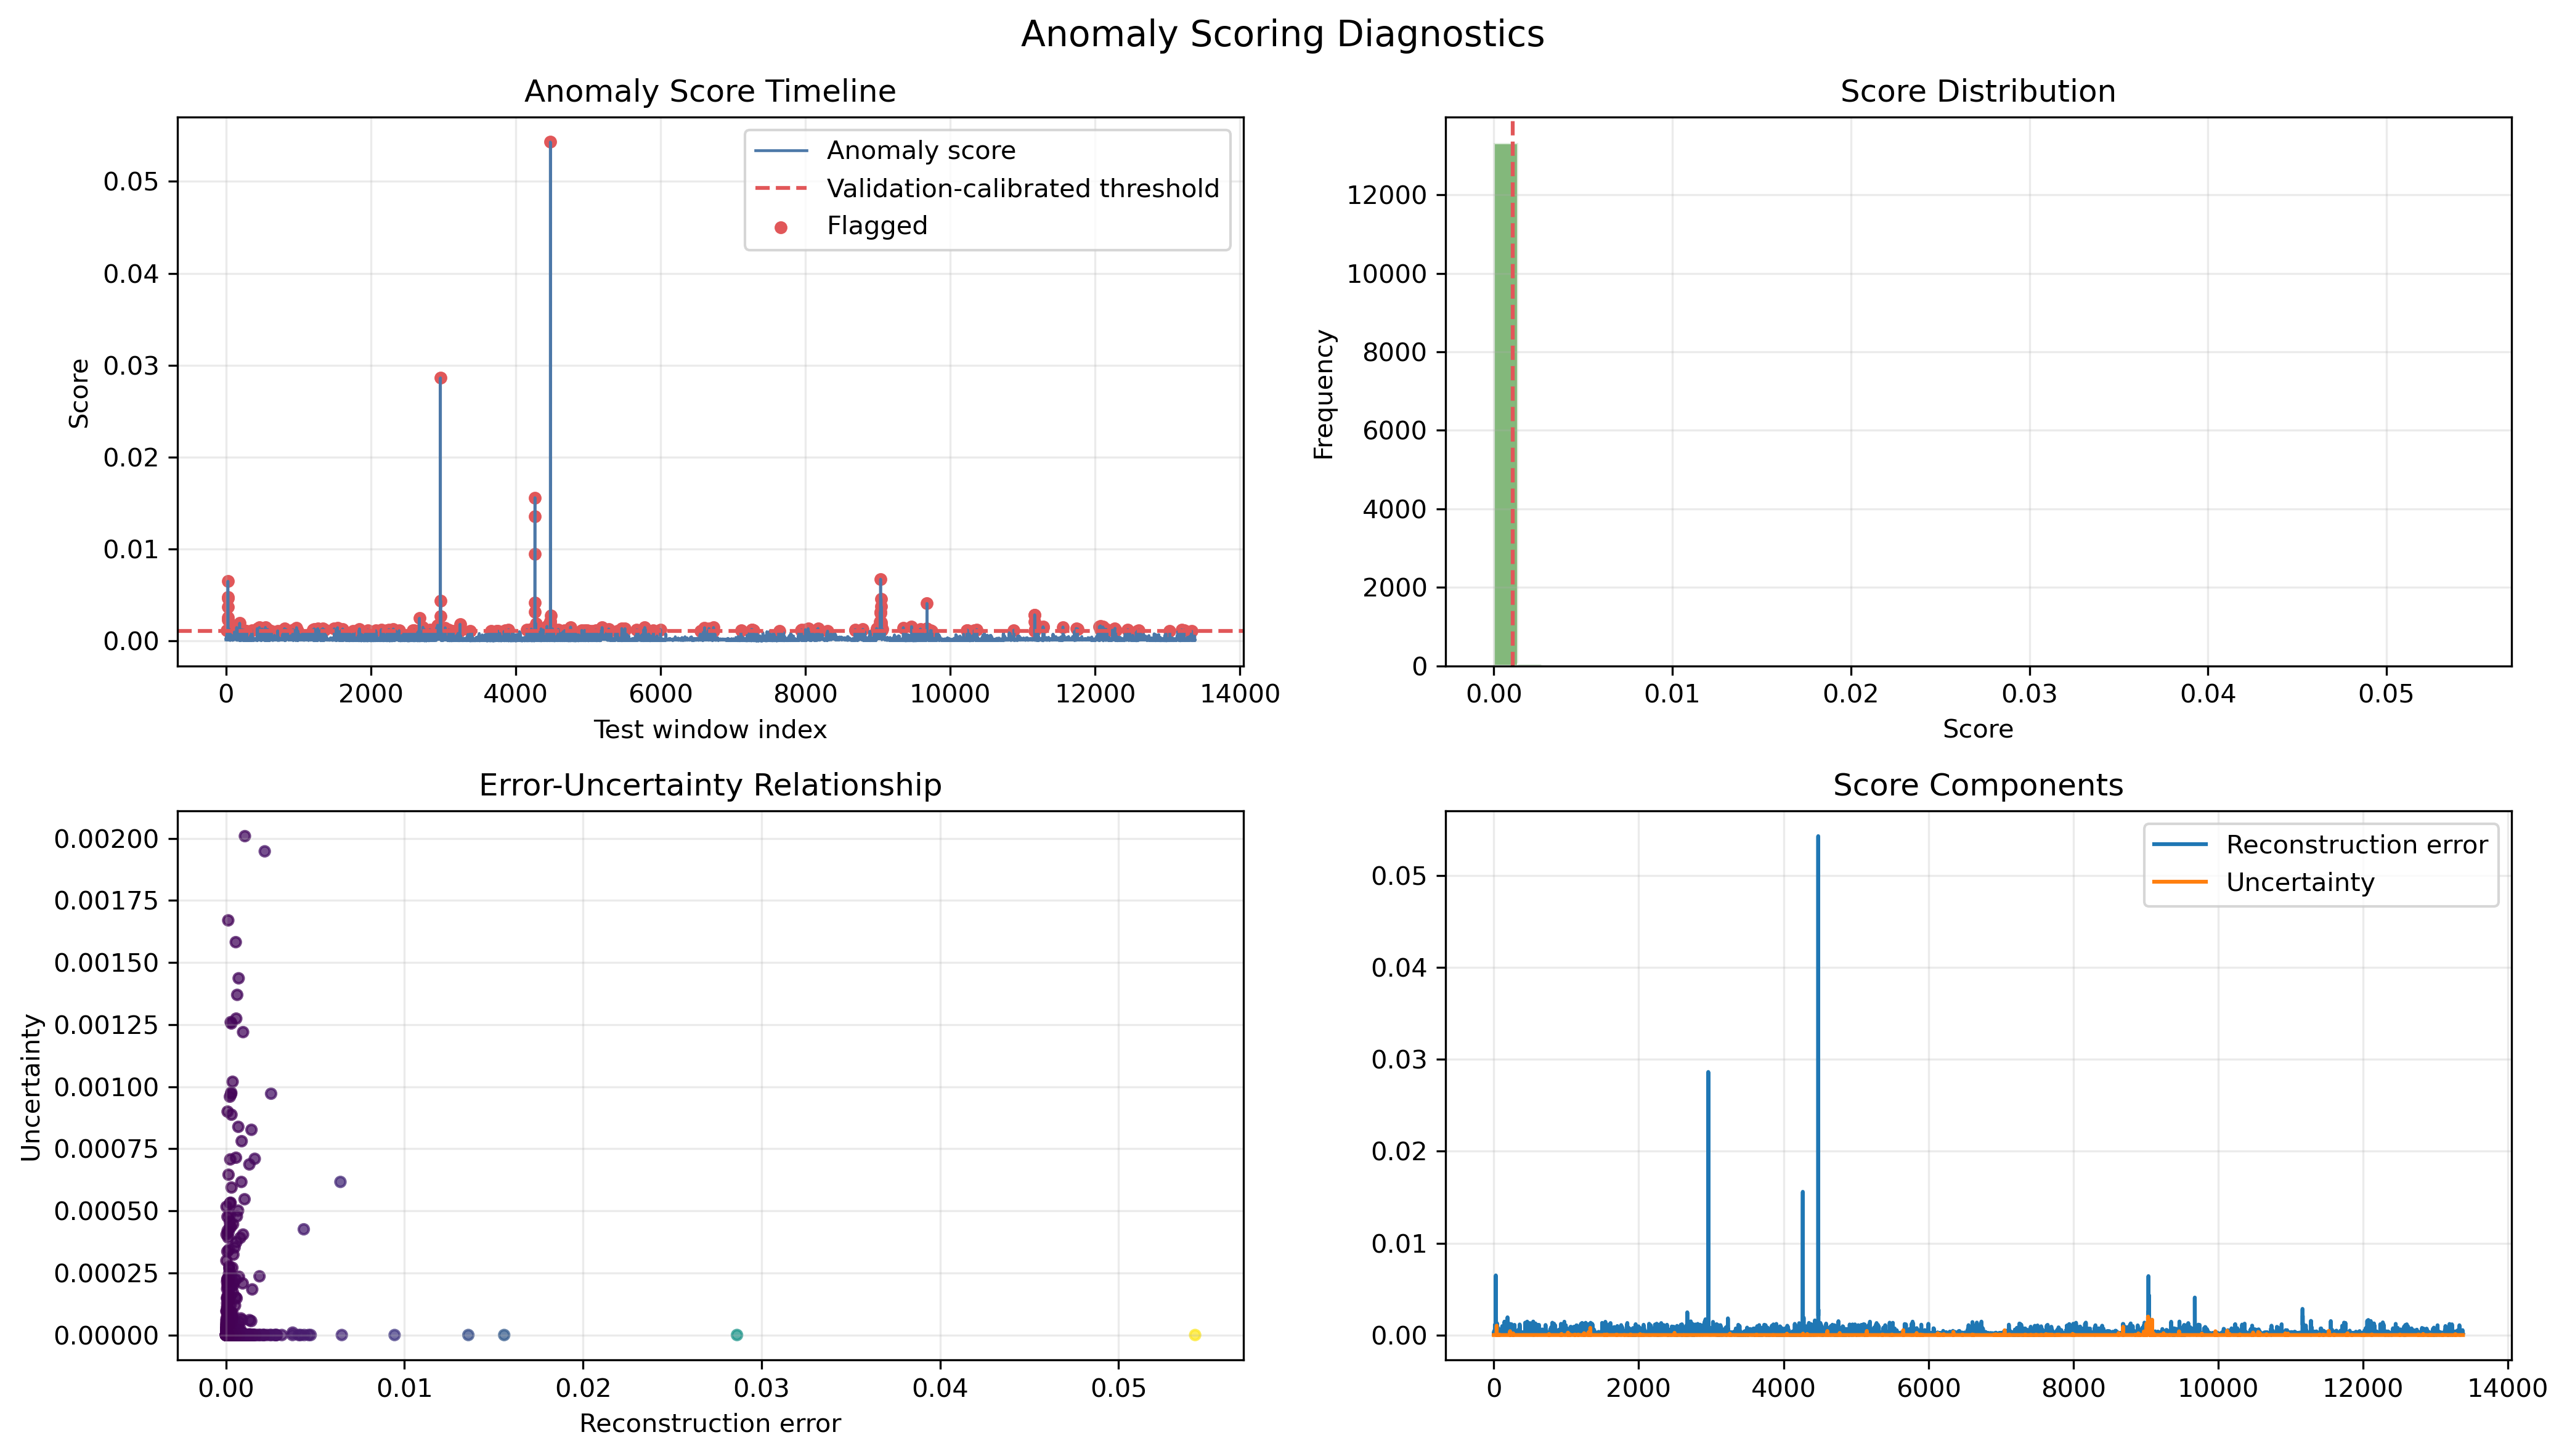
\includegraphics[width=\textwidth]{images/04_anomaly_diagnostics_base.png}\\[1pt]
{\small (a) Base TCN: $\tau_{95} = 1.06\times 10^{-3}$, 239 flagged (1.79\%).}\\[8pt]
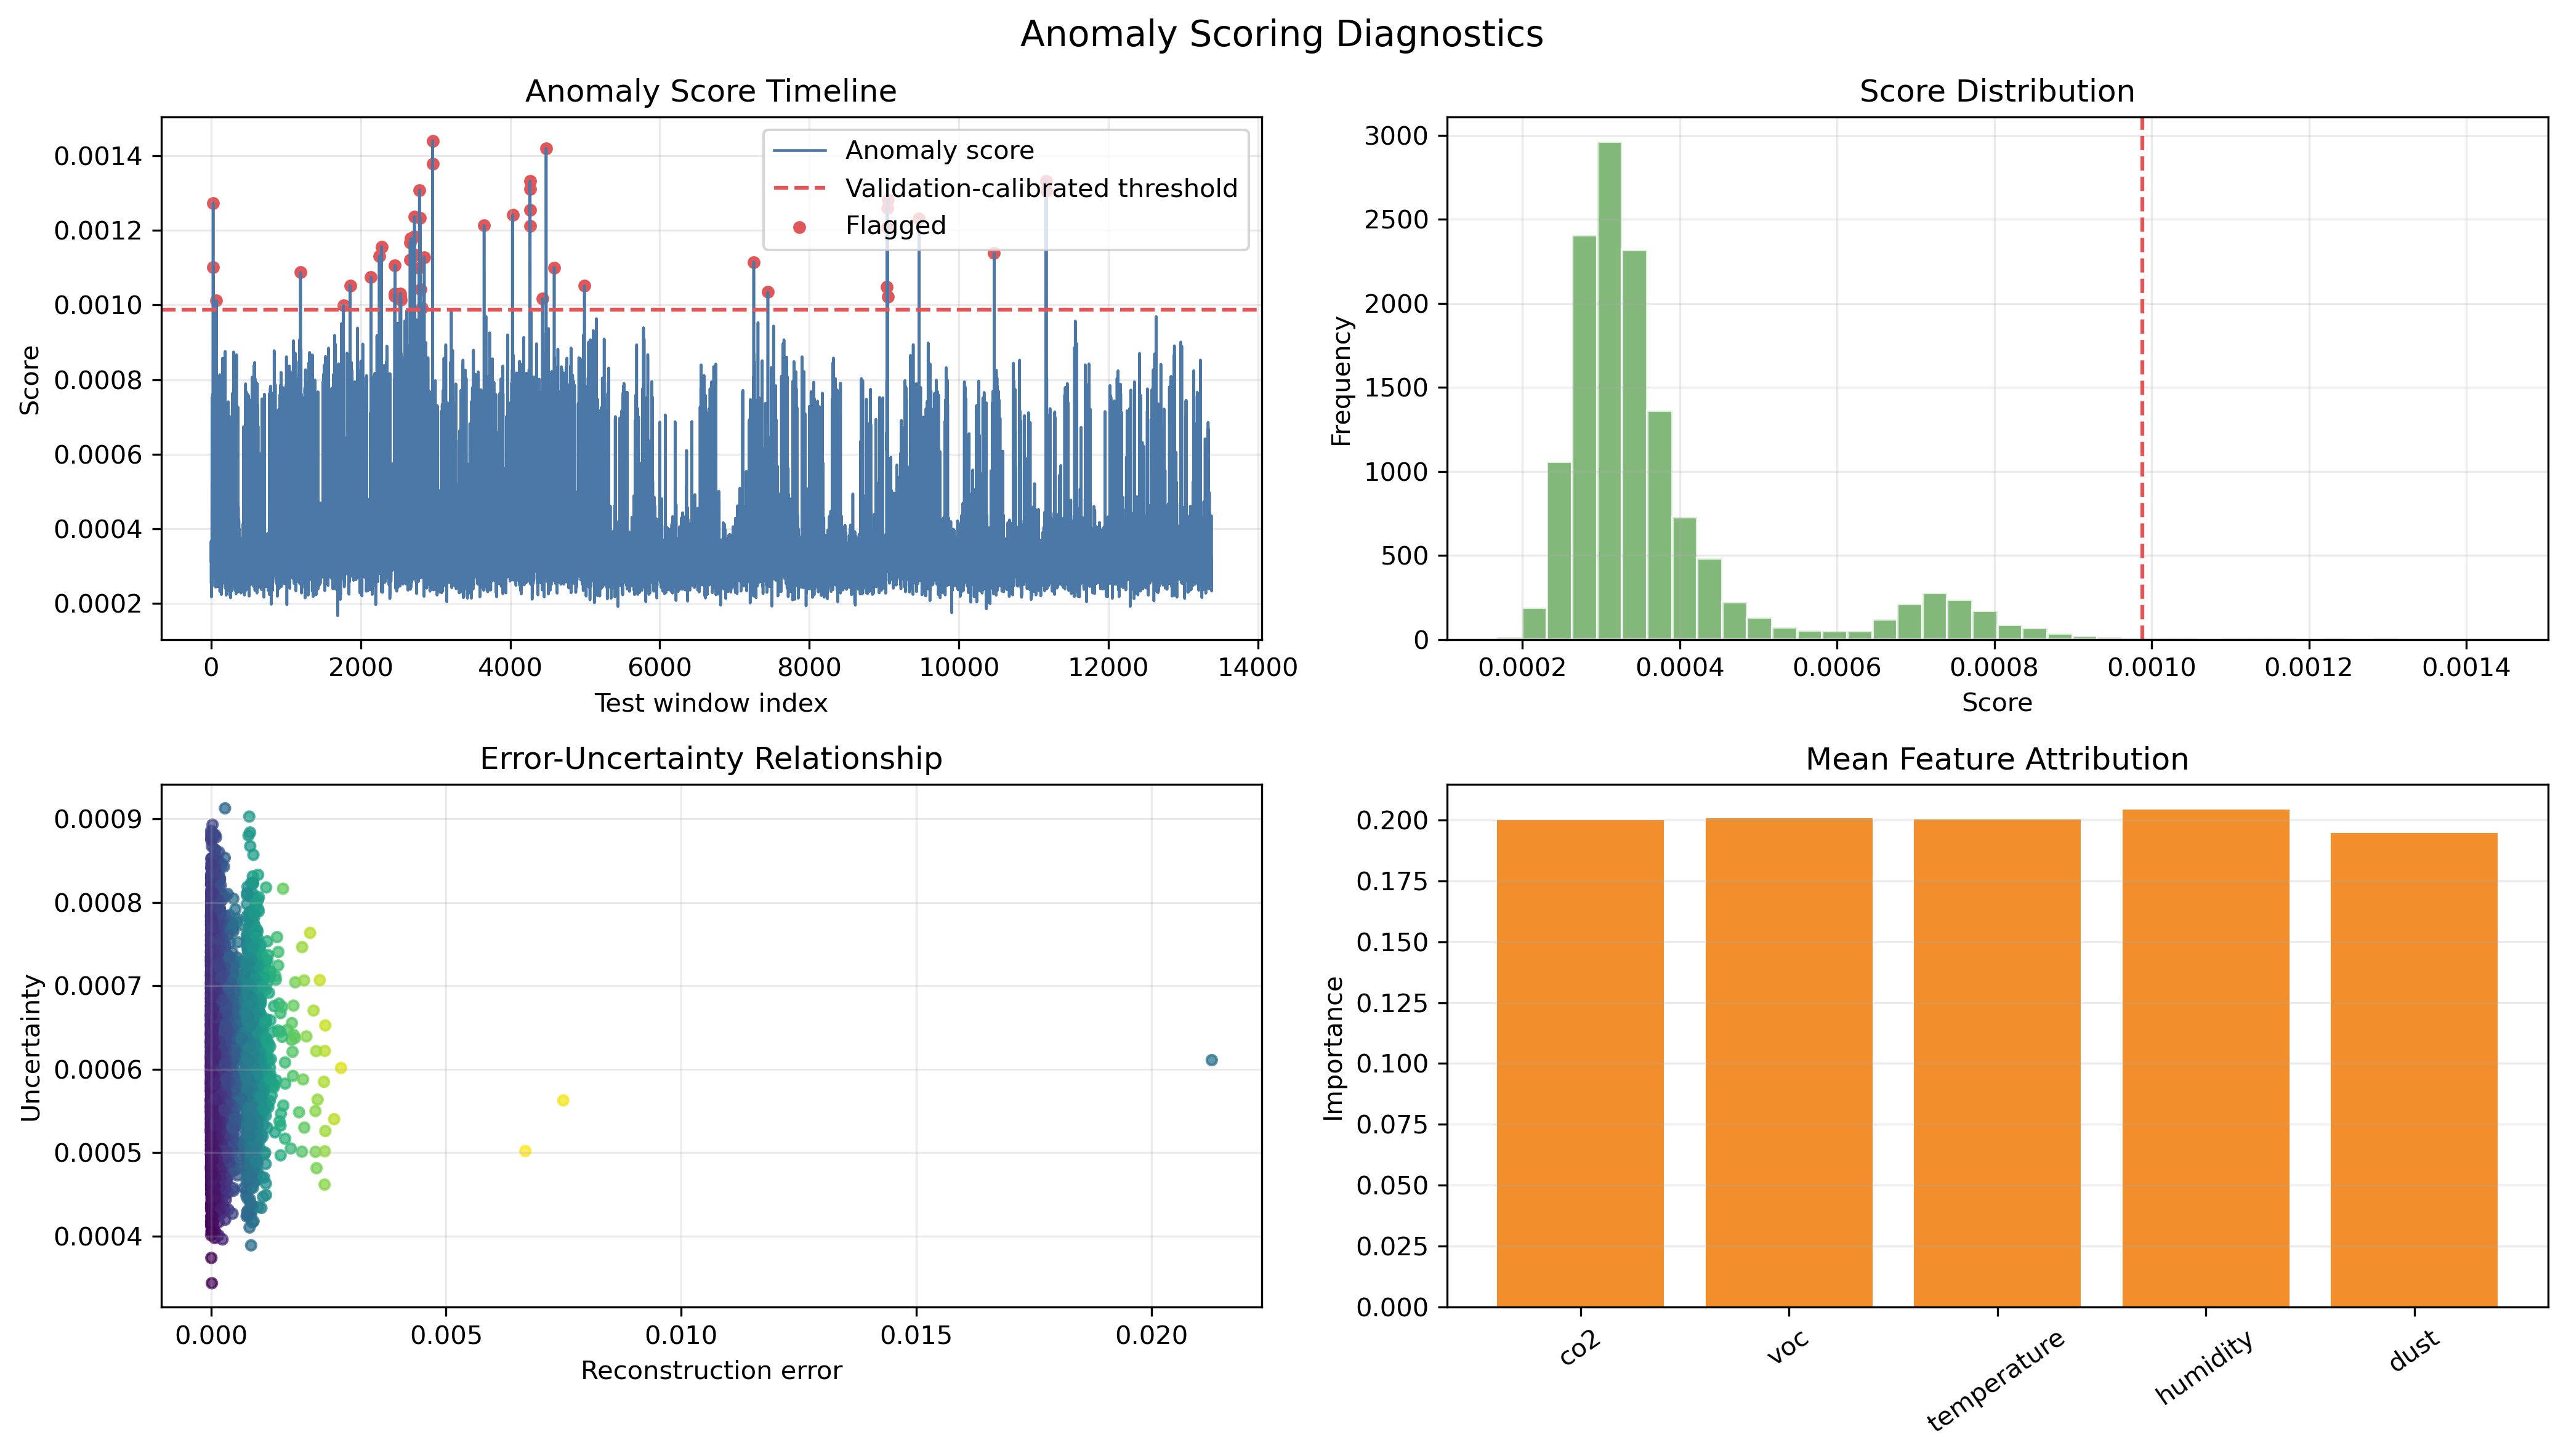
\includegraphics[width=\textwidth]{images/05_anomaly_diagnostics_enhanced.png}\\[1pt]
{\small (b) Full Enhanced (Proposed Model): $\tau_{95} = 9.93\times 10^{-4}$, 50 flagged (0.37\%).}
\caption{Anomaly detection diagnostics on the held-out test split for (a) Base TCN and (b) Full Enhanced, drawn with an identical four-panel layout and shared score axes for direct comparison: anomaly-score timeline (log $y$) with the validation-calibrated $\tau_{95}$ (dashed red) and flagged windows, score distribution (log $x$), error--uncertainty relationship (log--log), and per-sensor mean reconstruction error.}
\label{fig:anomaly_diagnostics}
\end{figure}

\subsection{Per-Sensor Attribution: Faithfulness Audit}

We treat the per-sensor attribution head as an \emph{exploratory} component and audit it rather than report it as a result. \cref{table:attribution} shows the attribution mass it assigns on the IAQ run---Humidity ($20.4\%$), VOC ($20.1\%$), CO\textsubscript{2} ($20.0\%$), Temperature ($20.0\%$), Dust ($19.5\%$)---which is essentially uniform. Such a flat distribution is not evidence that all sensors contribute equally; it is the signature of a head that fails to \emph{discriminate} among channels, as the audit below confirms.

\textbf{Controlled-perturbation faithfulness test.} We deliberately tested whether this near-uniform distribution reflects genuine per-sensor causal importance or merely an uninformative head, and we report the result candidly. On the labelled SKAB stream we ran a controlled-spike test: a $+6\sigma$ impulse was injected into one known channel of otherwise-normal windows, and we measured how often the learner's top-ranked channel matched the spiked one. The top-1 hit rate was only $0.127$, essentially at the random-chance level ($1/8 = 0.125$); the head collapses onto a single channel (it returned ``Voltage'' on $99.6\%$ of windows regardless of which channel was perturbed), and its attribution vector is not positively aligned with the per-channel reconstruction error on real anomalies (Spearman $\rho = -0.64$, $p = 0.09$). We therefore do \emph{not} claim that the attribution head provides validated, causally faithful explanations. The near-uniform IAQ distribution in \cref{table:attribution} should be read as the head failing to discriminate among channels rather than as evidence that all sensors contribute equally. We retain the module because it is trained jointly at negligible cost and the architecture supports attribution in principle, but making these attributions faithful (e.g.\ via gradient-based or perturbation-consistent attribution objectives) is an explicit direction for future work, not a present claim. The detection and uncertainty contributions of the framework do not depend on this head.

\begin{table}[H]
\centering
\caption{Attribution mass assigned by the feature-importance head on the IAQ run. The near-uniform distribution indicates the head does not discriminate among channels (see the faithfulness audit), and is reported as a diagnostic of this limitation rather than as a per-sensor importance result.}
\label{table:attribution}
\begin{tabular}{lc}
\toprule
\textbf{Sensor} & \textbf{Attribution} \\
\midrule
Humidity & 20.4\% \\
VOC & 20.1\% \\
CO\textsubscript{2} & 20.0\% \\
Temperature & 20.0\% \\
Dust (PM\textsubscript{2.5}) & 19.5\% \\
\bottomrule
\end{tabular}
\end{table}

\subsection{Additional Analyses}

\textbf{Computational Cost, Latency, and Scalability.} The Proposed model adds approximately 15\% more parameters relative to the Base TCN, primarily from the AUAA module (4 attention heads, 64-dim hidden) and the Dynamic Weight Adapter (context GRU, learned gating). \cref{table:latency_cost} reports measured inference cost on an NVIDIA GeForce GTX 1080 Ti with windows scored in a batch and the latency \emph{including} the full Monte-Carlo uncertainty pass. Per-window scoring latency scales linearly in $M$: $0.16$\,ms/window at the deployment budget $M=20$ and $0.29$\,ms/window at $M=50$, i.e.\ Monte-Carlo sampling is the dominant but still modest cost and is trivially parallel across the $M$ passes. A scalability probe over synthetic channel counts shows the convolutional backbone scales sub-linearly with the number of sensors, remaining under $1.2$\,ms/window up to $128$ channels. The principal cost driver for very high-rate or edge deployment is therefore the MC budget, which \cref{table:skab_msensitivity} shows can be reduced to $M=5$--$10$ with negligible detection loss; further reduction (single-pass distillation of the MC ensemble) is a natural edge-deployment route.

\begin{table}[H]
\centering
\caption{Measured inference cost (NVIDIA GeForce GTX 1080 Ti; latency includes the full Monte-Carlo pass). \textbf{Left:} per-window latency and F1 versus MC budget $M$ (8-channel SKAB). \textbf{Right:} per-window latency at $M=20$ versus sensor count $C$ (synthetic).}
\label{table:latency_cost}
\setlength{\tabcolsep}{8pt}\small
\begin{minipage}[t]{0.48\linewidth}\centering
\begin{tabular}{ccc}
\toprule
\textbf{$M$} & \textbf{ms/window} & \textbf{F1} \\
\midrule
5  & 0.023 & 0.476 \\
10 & 0.076 & 0.477 \\
20 & 0.162 & 0.477 \\
50 & 0.286 & 0.477 \\
\bottomrule
\end{tabular}
\end{minipage}\hfill
\begin{minipage}[t]{0.48\linewidth}\centering
\begin{tabular}{cc}
\toprule
\textbf{Channels $C$} & \textbf{ms/window ($M{=}20$)} \\
\midrule
8   & 1.06 \\
16  & 1.16 \\
32  & 0.76 \\
64  & 0.36 \\
128 & 0.37 \\
\bottomrule
\end{tabular}
\end{minipage}
\end{table}


\textbf{Robustness to sensor failures and noise.} Physical deployments suffer dropped sensor streams and noisy channels, so we stress-test the detector with its \emph{clean}-calibrated $\tau_{95}$ held fixed (\cref{table:skab_robustness}). Zeroing any single channel (a missing/failed stream) changes F1 by at most $0.006$, and injecting Gaussian noise up to $\sigma=1.0$ (standardized units) leaves F1 within $[0.475, 0.477]$. The multi-sensor fusion and uncertainty gating thus degrade gracefully rather than collapsing when an individual channel is corrupted. We did not test adversarial perturbations or inter-sensor time-synchronization errors; these remain open robustness questions for deployment.

\begin{table}[H]
\centering
\caption{Robustness on the SKAB test split with the clean-calibrated $\tau_{95}$ held fixed. Zeroing any single channel (a missing stream) or adding Gaussian noise up to $\sigma=1.0$ (standardized units) changes F1 by at most $0.006$.}
\label{table:skab_robustness}
\setlength{\tabcolsep}{7pt}\small
\begin{tabular}{lccc}
\toprule
\textbf{Condition} & \textbf{Precision} & \textbf{Recall} & \textbf{F1} \\
\midrule
Clean (reference)            & 0.556 & 0.417 & 0.477 \\
\midrule
Mask Accelerometer1RMS       & 0.556 & 0.417 & 0.477 \\
Mask Accelerometer2RMS       & 0.557 & 0.419 & 0.479 \\
Mask Current                 & 0.556 & 0.417 & 0.476 \\
Mask Voltage                 & 0.555 & 0.416 & 0.476 \\
Mask Pressure                & 0.556 & 0.418 & 0.477 \\
Mask Temperature             & 0.556 & 0.416 & 0.476 \\
Mask Thermocouple            & 0.556 & 0.416 & 0.476 \\
Mask Volume Flow RateRMS     & 0.555 & 0.426 & 0.482 \\
\midrule
Gaussian noise $\sigma=0.10$ & 0.556 & 0.416 & 0.476 \\
Gaussian noise $\sigma=0.25$ & 0.556 & 0.417 & 0.477 \\
Gaussian noise $\sigma=0.50$ & 0.555 & 0.416 & 0.475 \\
Gaussian noise $\sigma=1.00$ & 0.555 & 0.416 & 0.475 \\
\bottomrule
\end{tabular}
\end{table}


\textbf{Empirical calibration of the Chebyshev bound.} A distribution-free bound is only useful if it is respected in practice and not vacuously loose. \cref{table:chebyshev_calib} reports, on the SKAB normal validation windows, the observed false-positive rate at $\tau=\bar{s}+k\sigma_s$ against the guarantee $1/k^2$. The empirical rate stays below the bound at every $k$ (e.g.\ at the design point $k=4.47$ the bound is $0.05$ and the observed rate is $0.000$). On this corpus the score distribution is close to Gaussian (skewness $-0.23$, excess kurtosis $0.11$), so the bound is conservative, yet it remains the correct tool precisely because it stays valid without distributional assumptions: under the heavy-tailed or skewed score distributions that arise on other sensor corpora the Gaussian/percentile thresholds lose their coverage guarantee while the Chebyshev threshold does not. We therefore present it as a safe \emph{worst-case} operating point to be used alongside, not instead of, the empirical percentile threshold.

\begin{table}[H]
\centering
\caption{Empirical validation of the Chebyshev false-positive bound on the SKAB clean validation windows ($n=6190$). The observed false-positive rate at $\tau=\bar{s}+k\sigma_s$ stays below the distribution-free guarantee $1/k^2$ at every $k$.}
\label{table:chebyshev_calib}
\setlength{\tabcolsep}{8pt}\small
\begin{tabular}{ccc}
\toprule
\textbf{$k$} & \textbf{Bound $1/k^2$} & \textbf{Empirical FP rate} \\
\midrule
1.00 & 1.0000 & 0.15283 \\
1.50 & 0.4444 & 0.05945 \\
2.00 & 0.2500 & 0.01858 \\
3.00 & 0.1111 & 0.00032 \\
4.00 & 0.0625 & 0.00000 \\
4.47 & 0.0500 & 0.00000 \\
5.00 & 0.0400 & 0.00000 \\
\bottomrule
\end{tabular}
\end{table}


\textbf{Choice of uncertainty estimator.} MC dropout is one of several uncertainty-quantification options. To check that it is not a limiting choice, we compared it against a five-member deep ensemble of the forecaster under the identical hybrid-scoring protocol: the ensemble reaches F1 $0.110$ / ROC-AUC $0.685$ on SKAB, comparable to the single-model MC-dropout detector at the same (Base-TCN) architecture level (Base TCN, F1 $0.113$), while requiring $5\times$ the training and storage. This indicates that the detection gains in our framework come from the uncertainty-\emph{aware architecture} (AUAA and the dynamic weight adapter), not from the particular uncertainty estimator, and that MC dropout is the cost-efficient choice (a single model, $M$ trivially-parallel passes). Variational inference and evidential heads would require architectural changes and are known to be calibration-sensitive, while conformal prediction is complementary and is already reflected in our distribution-free Chebyshev threshold; we leave a full estimator sweep to future work.

\textbf{MC Sample Sensitivity.} The full evaluation reported above uses $M=50$ Monte Carlo samples; the sensitivity table in \cref{table:mc_sensitivity} reports indicative MSE values at smaller $M$ obtained by drawing the first $M$ samples from the same ensemble. Performance converges around $M \approx 20$, beyond which marginal gains plateau while computational cost scales linearly. For operational deployment with a 1-minute sensor sampling cycle we recommend $M=20$ (per-batch latency $<30$~ms), and $M=50$ for offline evaluation where calibration is the priority.

To confirm that this two-budget choice does not affect the \emph{detection} conclusions, \cref{table:skab_msensitivity} re-runs the SKAB evaluation at $M\in\{5,10,20,50\}$ and reports precision/recall/F1/ROC-AUC. The proposed model's F1 is essentially invariant ($0.476$--$0.477$ across all $M$) and its ROC-AUC rises by only $0.003$ from $M=20$ to $M=50$; the deployment budget $M=20$ therefore incurs no meaningful detection penalty. We use $M=50$ for the IAQ \emph{forecasting/calibration} numbers (where the predictive variance enters the uncertainty-calibration loss and the reliability diagram) and $M=20$ for the deployment-faithful detection benchmark; \cref{table:skab_msensitivity} shows the two budgets are interchangeable for detection, so the choice is one of latency rather than accuracy.

\begin{table}[H]
\centering
\caption{SKAB detection metrics versus the Monte-Carlo budget $M$ (seed 42, validation-calibrated $\tau_{95}$). F1 is essentially invariant to $M$ and ROC-AUC rises only $+0.003$ from $M=20$ to $M=50$.}
\label{table:skab_msensitivity}
\setlength{\tabcolsep}{6pt}\small
\begin{tabular}{lcccc}
\toprule
 & \multicolumn{2}{c}{\textbf{Base TCN}} & \multicolumn{2}{c}{\textbf{Full Enhanced}} \\
\cmidrule(lr){2-3}\cmidrule(lr){4-5}
\textbf{$M$} & \textbf{F1} & \textbf{ROC-AUC} & \textbf{F1} & \textbf{ROC-AUC} \\
\midrule
5  & 0.046 & 0.676 & 0.476 & 0.723 \\
10 & 0.063 & 0.677 & 0.477 & 0.725 \\
20 & 0.054 & 0.678 & \textbf{0.477} & 0.727 \\
50 & 0.061 & 0.679 & 0.477 & 0.730 \\
\bottomrule
\end{tabular}
\end{table}


\begin{table}[H]
\centering
\caption{Monte Carlo sample-count sensitivity of the Full Enhanced model's forecasting MSE and $R^2$ on the held-out \textbf{IAQ} test split (truncated subsets of the same $M=50$ ensemble; relative-time figures are forward-pass cost scaled with $M$).}
\label{table:mc_sensitivity}
\begin{tabular}{lccc}
\toprule
\textbf{$M$ Samples} & \textbf{MSE} & \textbf{R\textsuperscript{2}} & \textbf{Relative time} \\
\midrule
5   & $1.85\times 10^{-4}$ & 0.9986 & 0.10$\times$ \\
10  & $1.74\times 10^{-4}$ & 0.9987 & 0.20$\times$ \\
20  & $1.68\times 10^{-4}$ & 0.9988 & 0.40$\times$ \\
50  & $1.65\times 10^{-4}$ & 0.9988 & 1.00$\times$ \\
\bottomrule
\end{tabular}
\end{table}

\textbf{Threshold Comparison.} Three threshold methods produce different operating points on the test set with validation-calibrated parameters. The percentile method yields $\tau_{95} = 1.06\times 10^{-3}$ for the Base model and $\tau_{95} = 9.93\times 10^{-4}$ for the Proposed model. The adaptive threshold $\tau_{\text{adapt}} = \tau_{\text{base}} \cdot (0.8 + 0.4\bar{\alpha})$ with $\bar{\alpha} = 0.527$ produces a slightly higher operating point ($1.07\times 10^{-3}$ and $1.00\times 10^{-3}$ respectively). The Chebyshev threshold with $k = \sqrt{1/0.05} \approx 4.47$ provides distribution-free FP-rate control with the guarantee $P(\text{FP}) \leq 1/k^2 = 0.05$. The Chebyshev bound is conservative (no Gaussian assumption is made on the score distribution), offering a principled operating point for safety-critical deployments where false alarms carry high operational cost.